\chapter[Double-Track Maneuver Optimization]{Maneuver with DT for hairpin 4\textsuperscript{th} degree super ellipse, without LT or WT.}

In addition to the double-track (DT) model equations state equations,
% \begin{align*}
%     \dot X_p &= v_x\,\cos(\psi) - v_y\,\sin(\psi),\\
%     \dot Y_p &= v_x\,\sin(\psi) + v_y\,\cos(\psi),\\
%     \dot \psi &= r,\\
%     \dot v_x &= \frac{F_x}{m} + v_y\,r,\\
%     \dot v_Y &= \frac{F_Y}{m} + v_x\,r,\\
%     \dot r &= \frac{M_z}{I_{zz}}.
% \end{align*}
the input forces are filtered using a low pass filter with a time constant $\tau_f$ to prevent NaN errors during the optimization.
\begin{align}
    \dot F_{x(f)} &= \frac{1}{\tau_f}\,\left(F_{x(f)}^* - F_{x(f)}\right),\\
    \dot F_{x(r)} &= \frac{1}{\tau_f}\,\left(F_{x(r)}^* - F_{x(r)}\right),
\end{align}
where $F_{x(f)}^*$ and $F_{x(r)}^*$ are the inputs to the model.

The hairpin is modeled as two ellipses,
\begin{align}
    \frac{x}{R_1^i} + \frac{y}{R_2^i} & \geq 1, & \frac{x}{R_1^o} + \frac{y}{R_2^o} & \leq 1.
    % \frac{x}{R_1^î} + \frac{y}{R_2^i} &\geq 1 \ \text{Inner ellipse},
    % \frac{x}{R_1^o} + \frac{y}{R_2^o} &\leq 1 \ \text{outer ellipse}.
\end{align}
A straightforward model of combined forces is based on the friction ellipses and the Magic Formula. The tire parameters are taken from Berntorp, Karl, et al. "Models and methodology for optimal trajectory generation in safety-critical road–vehicle manoeuvres." Vehicle System Dynamics 52.10 (2014): 1304-1332.

The nominal normal force $F_z$ resting on the respective wheel in the steady state is given by
\begin{align}
    F_{z(1)} &= \frac{1}{2}\,mg\frac{l_r}{l_f+l_r}, & F_{z(2)} &= \frac{1}{2}\,mg\frac{l_r}{l_f+l_r}, & F_{z(3)} &= \frac{1}{2}\,mg\frac{l_f}{l_f+l_r}, & F_{z(4)} &= \frac{1}{2}\,mg\frac{l_f}{l_f+l_r}.
\end{align}

\section{Constrains}
\begin{description}
    \item[$v_x > 0$] to avoid $\div$ by zero error while calculating the lateral slips, $\alpha$.
    \item[$-\delta_{max} \leq \delta \leq \delta_{max}$] steering angle limit.
    \item[$-\dot\delta_{max} \leq \dot\delta \leq \dot\delta_{max}$] steering angle rate limit.
    \item[$-\epsilon\,D_{x(f)} \leq F_{x(f)}^* \leq \epsilon\,D_{x(f)}$], limiting the forces on the front wheel, and $\epsilon$ is a number close to 1 to avoid NaN errors. 
    \item[$-\epsilon\,D_{x(r)} \leq F_{x(r)}^* \leq 0$], limiting the forces on the rear wheel.
    \item[$X_f - \beta \leq X_p(\text{end}) \leq X_f + \beta $], Allowing some error on the final $X_P$.
    \item[$Y_f - \beta \leq Y_p(\text{end}) \leq Y_f + \beta $], Allowing some error on the final $Y_P$.
\end{description}
The model is front-wheel driven but can brake on all four wheels.

\section{Cost function}
The const function $J$ is defined as 
\begin{align}
    J &= \min{\left(t + 0.5\beta\right)},
\end{align}
The number 0.5 is arbitrarily chosen. 

The vehicle parameters and constraints for the the optimal control problem are presented in Table \ref{tab:ocp_prob2}.

\begin{table}[h!]
    \begin{subtable}{0.3\textwidth}
        \begin{tabular}{c|c}
            parameter & value\\
            \hline
            $m$ & 2100\,kg\\
            $l_f$ & 1.3\,m \\     
            $l_r$ & s1.5\,m \\
            $w$ & 0.8\,m\\
            $g$ & 9.82\,m/s\textsuperscript{2}\\
            $I_{zz}$ & 3900\,kgm\textsuperscript{2}\\
        \end{tabular}
        \caption{Vehicle parameters}
    \end{subtable}
    \hfill
    \begin{subtable}{0.3\textwidth}
        \begin{tabular}{c|c}
            parameter & value\\
            \hline
            $R_1^i$ & 2\,m \\
            $R_2^i$ & 50\,m \\
            $R_1^o$ & 7\,m \\
            $R_2^o$ & 55\,m \\
        \end{tabular}
        \caption{Hairpin parameters}
    \end{subtable}
    \hfill
    \begin{subtable}{0.3\textwidth}
        \begin{tabular}{c|c}
            parameter & value\\
            \hline
            $\delta_{max}$ & 30$^\circ$ \\
            $\dot\delta_{max}$ & 45$^\circ$/s \\
            $\tau_f$ & 0.1\,s\\
            $\epsilon$ & 0.99\\
        \end{tabular}
        \caption{Constrains}
    \end{subtable}
    \caption{The vehicle, hairpin, and constraints for the DT-optimal vehicle Maneuver problem.}
    \label{tab:ocp_prob2}
\end{table}

The optimal trajectory for the DT model through the hairpin is presented in Figure~\ref{fig:DT_hairpin_path}. 

\begin{figure}[h!]
    \centering
    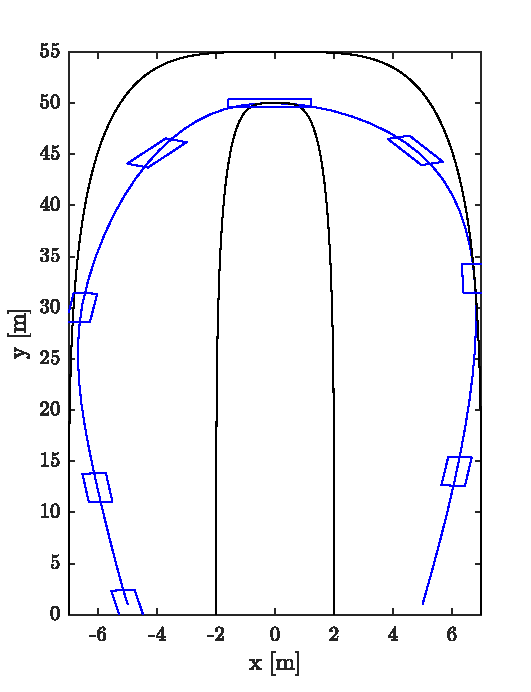
\includegraphics{figures/prob2_DT_path.pdf}
    \caption{Optimal trajectory for a harpin maneuver with minimum time for DT-model.}
    \label{fig:DT_hairpin_path}
\end{figure}

The states and forces acting on the wheels for the DT model for the hairpin are presented in Figure~\ref{fig:DT_hairpin_path_detail}. 

\begin{figure}[p]
    \centering
    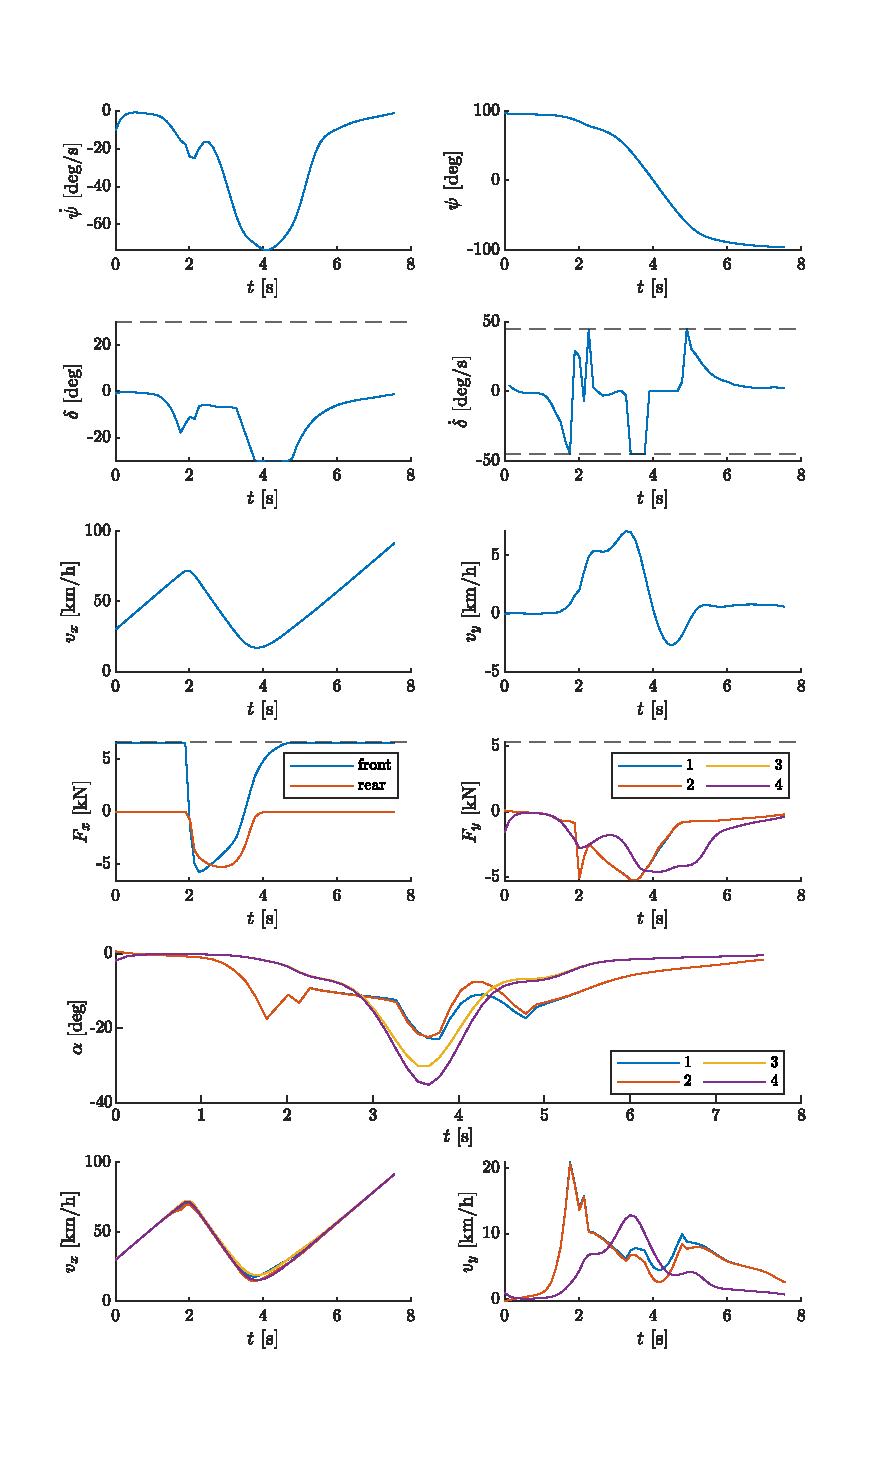
\includegraphics{figures/prob2_DT_path_detail.pdf}
    \caption{velocities, forces, and steering angels during the optimal trajectory for a harpin maneuver with minimum time for DT-model.}
    \label{fig:DT_hairpin_path_detail}
\end{figure}


\noindent\fbox{%
    \parbox{\textwidth}{%
        \textbf{Some reflections}: \newline
        The OCP for the DT model hairpin turn maneuver can have difficulty finding the optimal solution if the initial guesses are non-trivial. Therefore to improve convergence, the height of the hairpin was slowly increased, and the simulation results from the previous iterations were used as initializations for the next.
    }%
}

\section{Code}

The source codes for this problem can be found at \newline \href{https://github.com/arvba41/optimal_vehicle_maneuvers/tree/main/uppgift/ugf2}{https://github.com/arvba41/optimal\_vehicle\_maneuvers}.

% $\mathbf{v_x > 0}$, to avoid $\div$ by zero error while calculating the lateral slips, $\alpha$.\\
% $\mathbf{-\delta_{max} \leq \delta \leq \delta_{max}}$, steering angle limit.\\
% $\mathbf{-\dot\delta_{max} \leq \dot\delta \leq \dot\delta_{max}}$, steering angle limit.\\
% opti.subject_to(-deltamax<=delta<=deltamax);    % steering angle limit
% opti.subject_to(-ddeltamax<=ddelta<=ddeltamax); % steering rate limit

